\chapter{Problema 1}

\section{Multiplexer 16:1}

\subsection{Multiplexer indirizzabile 16:1}
Si chiede di progettare un multiplexer indirizzabile 16:1, utilizzando un approccio per composizione, utilizzando multiplexer 4:1.\\
Quindi quello che si vuole progettare è il multiplexer rappresentato come seguito.
\begin{figure}[H]
	\centering
	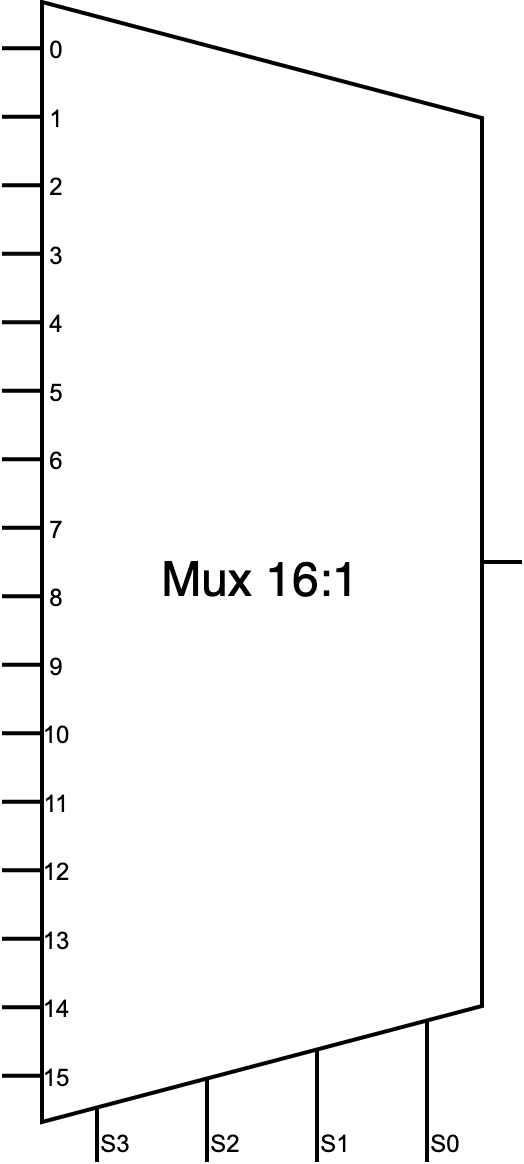
\includegraphics[width=0.2\textwidth]{img/01}
	\label{01} 
\end{figure}
Utilizzando l'approccio per composizione, si vuole dapprima progettare un multiplexer 4:1, utilizzando tre multiplexer 2:1.


\subsection{Rete di interconnessione a 16 ingressi e 4 uscite}

\subsection{Implementazione su board}

\section{Esercizio 1 - Sistema ROM+M}
